% Gambar 9. Alur model AI Glicovia (SVR tahap 1 dan SVM tahap 2).
% Kompilasi: pdflatex Gambar9_Alur_Model_AI.tex  (menghasilkan PDF vektor yang sudah terpotong rapi)
% Satu warna aksen (accent) hanya untuk dua model; sisanya skala abu-abu agar tetap terbaca bila dicetak hitam putih.
\documentclass[border=4pt]{standalone}
\usepackage[T1]{fontenc}
\usepackage{mathptmx}   % Times, seragam dengan teks paper
\usepackage{tikz}
\usetikzlibrary{arrows.meta,fit,calc}

\definecolor{ink}{HTML}{222222}
\definecolor{mid}{HTML}{6B6B6B}
\definecolor{accent}{HTML}{1F3A5F}

\begin{document}
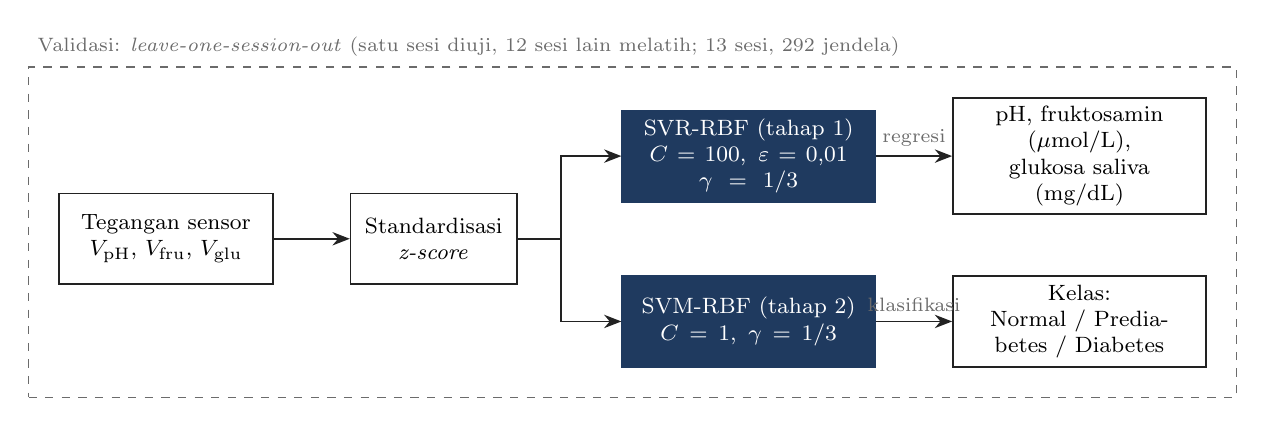
\begin{tikzpicture}[
  font=\footnotesize,
  >={Stealth[length=2.2mm,width=1.7mm]},
  line width=0.6pt,
  blk/.style={draw=ink, fill=white, minimum height=1.15cm, align=center, inner sep=3pt},
  mdl/.style={blk, draw=accent, fill=accent, text=white},
  arr/.style={->, draw=ink},
  note/.style={font=\scriptsize, text=mid, align=center}
]
  % --- simpul (koordinat dalam cm) ---
  \node[blk, text width=2.5cm] (in)  at (1.3, 0)    {Tegangan sensor\\ $V_{\mathrm{pH}},\,V_{\mathrm{fru}},\,V_{\mathrm{glu}}$};
  \node[blk, text width=1.9cm] (std) at (4.7, 0)    {Standardisasi\\ \textit{z-score}};
  \node[mdl, text width=3.0cm] (svr) at (8.7, 1.05)  {SVR-RBF (tahap 1)\\ $C=100,\ \varepsilon=0{,}01$\\ $\gamma=1/3$};
  \node[mdl, text width=3.0cm] (svm) at (8.7, -1.05) {SVM-RBF (tahap 2)\\ $C=1,\ \gamma=1/3$};
  \node[blk, text width=3.0cm] (o1)  at (12.9, 1.05)  {pH, fruktosamin ($\mu$mol/L),\\ glukosa saliva (mg/dL)};
  \node[blk, text width=3.0cm] (o2)  at (12.9, -1.05) {Kelas:\\ Normal / Prediabetes / Diabetes};

  % --- panah ---
  \draw[arr] (in) -- (std);
  \draw[arr] (std.east) -- ++(0.55,0) |- (svr.west);
  \draw[arr] (std.east) -- ++(0.55,0) |- (svm.west);
  \draw[arr] (svr) -- (o1);
  \draw[arr] (svm) -- (o2);

  % --- keterangan pada panah ---
  \node[note, above] at ($(svr.east)!0.5!(o1.west)$) {regresi};
  \node[note, above] at ($(svm.east)!0.5!(o2.west)$) {klasifikasi};

  % --- bingkai validasi ---
  \node[draw=mid, dashed, inner sep=0.38cm, fit=(in)(std)(svr)(svm)(o1)(o2)] (frame) {};
  \node[note, anchor=south west, align=left] at (frame.north west)
    {Validasi: \textit{leave-one-session-out} (satu sesi diuji, 12 sesi lain melatih; 13 sesi, 292 jendela)};
\end{tikzpicture}
\end{document}
